

%\newcommand*{\ACM}{}%

\ifdefined\ACM

%\documentclass[sigplan,screen]{acmart}
\documentclass[manuscript,screen,review]{acmart}

\else
 \documentclass[14pt]{article}
%\usepackage{libertine}
\usepackage{cuted}%\usepackage{widetext}
\usepackage[utf8]{inputenc}
\usepackage[a4paper, total={6in, 9in}]{geometry}
\usepackage{braket}
\usepackage{xcolor}
\usepackage{amsmath}
\usepackage{amsfonts}
\usepackage{amsthm}
\usepackage{amssymb}
%\usepackage[ocgcolorlinks]{hyperref}
\usepackage{hyperref}
%\usepackage{hyperref,xcolor}
%\usepackage[ocgcolorlinks]{ocgx2}
\usepackage{cleveref}
\usepackage{graphicx}
\usepackage{svg}
\usepackage{float}
\usepackage{tikz}
\usetikzlibrary{patterns, shapes.arrows}
\usepackage{adjustbox}
%\usepackage{tikz-network}
\usepackage{tkz-graph}
\usepackage{tkz-berge}
\usepackage[linesnumbered]{algorithm2e}
\usepackage{multicol}
\usepackage[backend=biber,style=alphabetic,sorting=ynt]{biblatex}
%\usepackage{xcolor}
%\usepackage{tkz-berge}
%\usepackage{tkz-graph}
\usepackage{pgfplots}
\usepackage{sagetex}
\usepackage{setspace}
\usepackage{etoc}
%\usepackage{wrapfig}
\usepackage{pgfgantt}
\DeclareUnicodeCharacter{2212}{−}
\usepgfplotslibrary{groupplots,dateplot}
\pgfplotsset{compat=newest}

\newtheorem{theorem}{Theorem}
\newtheorem{definition}{Definition}
\newtheorem{example}{Example}
\newtheorem{claim}{Claim}
\newtheorem{fact}{Fact}
\newtheorem{remark}{Remark}
\newtheorem*{theorem*}{Theorem}
\newtheorem{lemma}{Lemma}
\crefname{lemma}{Lemma}{Lemmas}
\hypersetup{colorlinks=true}
% , allcolors=blue,allbordercolors=blue,pdfborderstyle={0 0 1}}
%\hypersetup{pdfborder={2 2 2}}
% pdfpagemode=FullScreen,
% backref 

\newtheorem{problem}{Problem}
\crefname{problem}{Problem}{Problems}

\DeclareMathOperator{\Ima}{Im}


\usepackage{cancel}
\usepackage{subcaption}
\addbibresource{./sample.bib}

\fi

\begin{document}
\newcommand{\commentt}[1]{\textcolor{blue}{ \textbf{[COMMENT]} #1}}
\newcommand{\ctt}[1]{\commentt{#1}}
\newcommand{\prb}[1]{ \mathbf{Pr} \left[ #1 \right]}
\newcommand{\prbm}[2]{ \mathbf{Pr}_{ #2 }\left[ #1 \right]}
\newcommand{\prbc}[3]{ \mathbf{Pr}_{ #2 }\left[ #1 \right | #3]}
\newcommand{\prbcprb}[3]{ \prbc{#2}{#1}{#3} \cdot \prb{#3} } 
\newcommand{\expp}[1]{ \mathbf{E} \left[ {#1} \right]}
\newcommand{\onotation}[1]{\(\mathcal{O} \left( {#1}  \right) \)}
\newcommand{\ona}[1]{\onotation{#1}}
\newcommand{\PSI}{{\ket{\psi}}}
\newcommand{\xij} { X_{ij} } 
\DeclareMathOperator{\Ima}{Im}
%\newcommand{\LESn}{\ket{\psi_n}}
%\newcommand{\LESa}{\ket{\phi_n}}
%\newcommand{\LESs}{\frac{1}{\sqrt{n}}\sum_{i}{\ket{\left(0^{i}10^{n-i}\right)^{n}}}}
%\newcommand{\Hn}{\mathcal{H}_{n}}
%\newcommand{\Ep}{\frac{1}{\sqrt{2^n}}\sum^{2^n}_{x}{ \ket{xx}}}
%\newcommand{\HON}{\ket{\psi_{\text{honest}}}}
%\newcommand{\Lemma}{\paragraph{Lemma.}}
\newcommand{\Cpa}{[n, \rho n, \delta n]}
%\setlength{\columnsep}{0.6cm}
\newcommand{\Jvv}{ \bar{J_{v}} } 
\newcommand{\Cvv}{ \tilde{C_{v}} } 

\newcommand{\Gz}{ G_{z}^{\delta} } 
\newcommand{ \Tann } {  \mathcal{T}\left( G, C_0 \right) }
\newcommand{\ireducable}{ireducable \hyperref[ire]{[\ref{ire}]} }
\newcommand{\cutUU}{E(U_{-1} \bigcup U_{+1} ,U)} 
\newcommand{\wcutUU}{w\left( E(U_{-1} \bigcup U_{+1} ,U)  \right)}
\newcommand{\testgo}{  \mathcal{T}\left(J, q , C_{0}\right) } 

\newcommand{\duC}{\left( C_{A}^{\perp}\otimes C_{B}^{\perp} \right)^{\perp}}
\newcommand{\duduC}{\left( C_{A}\otimes C_{B}\right)^{\perp}}
  




%\title{ $\textbf{QNC}_{1} \subset $ noisy-\textbf{BQP}}
\title{ Research Proposal - Fault-Tolerainzing Shallow Circuits. }
\author{Michael Ben-Or \ \ David Ponarovsky}
\maketitle

\newcommand*{\Mbas}{\mathcal{X}^\prime}
\newcommand*{\bas}{\mathcal{X}}
\newcommand*{\sMbas}{\Mbas}
\newcommand*{\QQ}{C_{X}/C_{Z}^\perp }
\newcommand*{\trig}{ Triorthogonal }
\newcommand*{\Hyp}{ Hyperproduct }
\newcommand*{\Cin}{ C_{\text{initial}} }
\newcommand*{\Ctan}{ C_{\text{Tan}} }



\newcommand*{\QACze}{\mathbf{QAC}_{0}}
\newcommand*{\QNCzef}{\mathbf{QNC}_{0,f}}
\newcommand*{\QNCze}{\mathbf{QNC}_{0}}
\newcommand*{\QNCon}{\mathbf{QNC}_{1}}
\newcommand*{\NCon}{\mathbf{NC}_{1}}
\newcommand*{\noiseQNCon}{noisy-$\QNCon$}
\newcommand*{\QNC}{\mathbf{QNC}}
\newcommand*{\QNCG}{\mathbf{QNC_G}}
\newcommand*{\NC}{\mathbf{NC}}
\newcommand*{\QNCiG}{\mathbf{QNC_{G,i}}}


% Constant depth fault tolerance construction.   
\newcommand*{\CDO} {CDFT} 



\abstract{We study the overall depth overhead cost required for constructing fault-tolerant circuits. We focus on shallow depth circuit classes, in particular, $\QACze{}, \QNCzef{}$, $\QNCon{}$, and '$\QNC{}$ without reset gates', and certain known problem candidates for demonstrating quantum advantage such as factoring \cite{Shor_1997} and Instantaneous Quantum Polynomial-time \cite{Bremner_2017}, \cite{Paletta_2024}. We aim to answer whether there exists a fault tolerance with only constant overhead at the circuit's depth. A positive answer implies that computing logarithmic depth circuits when subjected to noise is not harder than computing in an ideal environment.

  \section{Introduction.} 
  
The Quantum Computation model is widely believed to be superior to classical models, offering asymptotic speedup in tasks such as factoring \cite{Shor_1997}, searching \cite{grover1996fast}, simulating, and more relative to the best-known classical solutions. Yet even though there is almost complete agreement about the superiority of the ideal quantum model, there is still a debate over whether it is possible to implement complex computation in the real world, where the qubits and gates are subject to faults. Similarly, the feasibility of realizing classical computation has also been an open question, In fact the question about the feasibility of computation under noise is almost as ancient as the computer science field itself, initialized by Von Neumann \cite{Neumann+1956+43+98} at the time that classical computation putted in debuts. Time been pass and the followed works had pointed that not even a polynomial computation in the presence of noise is still reasonable but one can implement a fault tolerance version at a most constant times cost at the circuits depth \cite{Pippenger}. Or in asymptotic sense, classical computation in the presence of noise is as exactly hard as computation in ideal environment.  

Recently, the feasibility question has been raised again, this time regarding quantum computing, and while an intensive work has been done, and also succeed to prove that polynomial quantum computation can be made fault tolerance, \cite{aharonov1999faulttolerant},\cite{gottesman2014faulttolerant} and even with only constant overhead at the original circuit width \cite{grospellier:tel-03364419}, the required depth over-head is still not well understood. We stress out that in all the familiar constructions, in construct to Pippenger \cite{Pippenger}, original constant-depth gates are mapped to asymptotically grow\footnote{Note, that here, classical computation is also counted in the overall depth cost} depth gates. 


Moreover, even the depth overhead is particularly interesting as today's quantum machines are challenged to maintain quantum states for a long time \cite{CITE}. The limitations of these machines have motivated research to define NISQ, which stands for Noisy Intermediate-Scale Quantum, referring to the current era of quantum computing characterized by quantum processors that have a limited number of qubits and are prone to errors due to noise. In addition to NISQ, another common characterization for limited quantum computation is computation without reset gates, which has been proved to be impossible when restricted to polynomial space \cite{aharonov1996limitationsnoisyreversiblecomputation}. Having a constant depth-overhead fault tolerance scheme would imply the feasibility of log depth computation in that model.
  
%This work address the above, We ask whether a magnitude depth overhead is an unavoidable price that one has to pay. And, in particular, whether an ideal $\QNCon$, the class of problem can be decided by logarithmic depth quntum circuits, can be computed in noisy-$\QNCon$ circuits. We show how using the ideas presented in \cite{grospellier:tel-03364419} and \cite{Pippenger} gives almost immediately $\QNCzef \subset$ \noiseQNCon and that sampling from IQP, Instantaneous Quantum Polynomial-time \cite{Bremner_2017}, \cite{Paletta_2024}, also can be done in logarithmic depth circuits.    
This work addresses the above. We ask whether a magnitude depth overhead is an unavoidable price that one has to pay, If a Constant Depth Fault Tolerance Construction (\CDO{}) exists, and if so, how to construct it. In particular, whether an ideal $\QNCon{}$, the class of problems that can be decided by logarithmic depth quantum circuits, can be computed in noisy-$\QNCon{}$ circuits.

Additionally, we extend the question beyond the standard classes and ask about fault-tolerant sampling. Specifically, we consider several sampling processes by shallow quantum circuits, which are believed to be infeasible for classical circuits, such as Instantaneous Quantum Polynomial-time \cite{Bremner_2017}, \cite{Paletta_2024}, and ask about the depth efficiency of their fault-tolerant version.

%$\QNCzef \subset$ \noiseQNCon 
%
%We show how using the ideas presented in \cite{grospellier:tel-03364419} and \cite{Pippenger} gives almost immediately $\QNCzef \subset$ \noiseQNCon and that sampling from IQP, , also can be done in logarithmic depth circuits.



  
  
The proposal is organized as follows. \Cref{sec:nota} presents the notations, formal definitions, and states the open problems that will be studied through the research. Then, \Cref{sec:opt} describes strategies to prove \CDO{}. In particular, it lists primitives that can be used to achieve it and discusses how far we are from obtaining them. Having said that, \Cref{sec:passi} presents the first cues against the possibility of \CDO{} and provides the entry points to prove the impossibility claim. Finally, \Cref{sec:app} discusses the applications and implications of either the correctness of \CDO{} or the impossibility of \CDO{}, from both theoretical and practical views.


  \section{ Notations. } \label{sec:nota}

  We use the standard notations commonly used in the literature. When not otherwise mentioned, we consider quantum states over qubits, each lying in a two-dimensional Hilbert space $\mathcal{H}_{2}$, and denote by $\mathcal{H}_{2^n}$ the Hilbert space of an $n$-qubit system. Pure quantum states and their dual presentations are denoted by $\ket{\psi}, \bra{\psi}$, and in the matrix representation, we use $\ket{\psi}\bra{\psi}$ to denote its density matrix. We will use $\rho$ to denote a mixed state, whose density matrix is a trace one PSD matrix. We use $\mathcal{N} : L(\mathcal{H}) \rightarrow L(\mathcal{H})$ to denote a $p$-local stochastic noise channel, namely a channel in which for any subset $S$ of the (qu)bits, the probability that all the qubits in $S$ absorb noise is less than $p^{|S|}$. We recall that for a constant-depth circuit, when the fanout/in of its subgates is bounded, one can map the running of the circuits subjected to $p$-local stochastic noise to a running when the states are subjected only to $p^{\prime}$-local stochastic noise before entering the circuit, and then the rest of the computation is done in an ideal environment \cite{gottesman2014faulttolerant}, where $p^{\prime}$ is a function of $p$ and constants. If the gate is also a measure, for example as a decoder, then the mapping induces also $q$-local stochastic noise on the measurements.

  \begin{figure}[h]
  \label{fig:noise}
  \begin{center}
  \begin{quantikz}[row sep=0.3cm, column sep=0.7cm]
    \lstick{$q_1$} & \gate[wires=8]{U_0} & \gate{\mathcal{N}} & \gate[wires=8]{U_1}   & \gate{\mathcal{N}} & \gate[wires=8]{U_2} & \gate{\mathcal{N}}& \qw \\
    \lstick{$q_2$} &                      & \gate{\mathcal{N}} &                      & \gate{\mathcal{N}} &                     & \gate{\mathcal{N}} & \qw \\
    \lstick{$q_3$} &                      & \gate{\mathcal{N}} &                      & \gate{\mathcal{N}} &                     & \gate{\mathcal{N}} & \qw \\
    \lstick{$q_4$} &                      & \gate{\mathcal{N}} &                      & \gate{\mathcal{N}} &                     & \gate{\mathcal{N}} & \qw \\
    \lstick{$q_5$} &                      & \gate{\mathcal{N}} &                      & \gate{\mathcal{N}} &                     & \gate{\mathcal{N}} & \qw \\
    \lstick{$q_6$} &                      & \gate{\mathcal{N}} &                      & \gate{\mathcal{N}} &                     & \gate{\mathcal{N}} & \qw \\
    \lstick{$q_7$} &                      & \gate{\mathcal{N}} &                      & \gate{\mathcal{N}} &                     & \gate{\mathcal{N}} & \qw \\
    \lstick{$q_8$} &                      & \gate{\mathcal{N}} &                      & \gate{\mathcal{N}} &                     & \gate{\mathcal{N}} & \qw
  \end{quantikz}
  \caption{ Circuit subjected to noise. }

  \end{center}
\end{figure}

We think about computation subjected to noise as the running of a circuit, in which at any time, qubits might be 'flipped', or formally, with some constant probability, they are replaced with the fully mixed state. Since our computation might create correlations between the errors, we will assume nothing about the behavior of the errors except that big errors are unlikely. By doing that, the induction step doesn't have to guarantee the errors being uncorrelated. 

We use \Cref{def:pnoise} to describe the running of a circuit subjected to noise. \Cref{fig:noise} illustrates a noisy circuit. In the figure, the channel $N$ acts on each qubit separately, yet this is not the case, and we impose it in that way only to make a clear distinction between the original gates and the noise channels. \begin{definition}{$p$-Noisy Circuit.}
    \label{def:pnoise}
    Given a circuit $C$ (regardless of the model), its $p$-noisy version $\tilde{C}$ is the circuit obtained by alternately taking layers from $C$ and then passing each (qu)bit through a $p$-local stochastic channel.
  \end{definition}

  
  Generally speaking, we say that a decision problem is solvable by a uniform family of circuits $\mathcal{C}$ if there is a polynomial $poly : \mathbb{R} \rightarrow \mathbb{R}$, such that for any large enough $n \in \mathbb{N}$, there exist $a, b \in (0,1)$ at a distance of at least $b - a > 1/\text{poly}(n)$ and a polynomial Turing machine $M$ such that for any given instance $x$ with encoding length $|x| = n$, the running of $M$ on $x$ outputs $C_x \in \mathcal{C}$ that, when running over the zero word $0^{*}$, induces on the first (qu)bit at least $b$ probability to be at $1$ if $x$ is in the language and at most $a$ to be at $1$ otherwise. 
If a decision problem is solvable by a $p$-noisy version of $C \in \mathcal{C}$, we say that the problem is solvable by noisy-$\mathcal{C}$. We abuse the notation, and for complexity class $Q$, we define noisy-$Q$ to be all the decision problems solvable by the noisy version of the circuit family that solves the problems in $Q$. For example, noisy-\textbf{BQP} is the class of all the decision problems solvable by noisy polynomial quantum circuits.  


The first class we are interested in is Nick's Class, $\NC{}$ \cite{CITE}, characterizing the boolean circuits at logarithmic depth. This class was proven by Pippenger to be equal to its noisy version, namely noisy-$\NC{} = \NC{}$ \cite{Pippenger}. Formally defined as follows: 
\begin{definition}[$\NC{}$ - Nick's Class]
$\NC_i$ is the class of decision problems solvable by a uniform family of Boolean circuits, with polynomial size, depth $O(\log^i(n))$, and fan-in $2$. 
\end{definition}


Second, the analog class of $\NC{}$ is $\QNC{}$, which characterizes logarithmic depth quantum circuits. In $\QNC{}$, the circuits are also allowed to have any single qubit gate. While in the classical case the number of functions from $\{0,1\} \rightarrow \{0,1\}$ is finite, in the quantum case we have an infinite number of single gates. That motivated us to define $\QNCG{}$ - the circuits when the gate set is restricted to some finite, constant size group $G$. We emphasize that in \textbf{BQP} there is no point in restricting to such a family since any gate can be polynomially approximated at polylogarithmic depth, so in that case, the restriction does not change computational power and one can assume to be able to apply any single qubit gate. However, when considering shallow circuits at logarithmic depth, such assumptions don't hold anymore.
\begin{definition}[$\QNC{}$]
  The class of decision problems solvable by polynomial size,  polylogarithmic-depth,  and finate fan out/in quantum circuits with bounded probability of error. Similarly to $\NC_i{}$, $\QNC_i{}$ is the class where the decisdes the circuits have $\log^i (n)$ depth.  
\end{definition}

\begin{definition}[$\QNCG{}$]
  For a fixing finate fan in/out gateset $G$, the class with deciding circuits at polynomial size, composed only for gates in $G$ and at depth at most polylogaritmic. And in similar to $\QNC_{i}{}$, $\QNCiG{}$ is the restriction to circuits with depth at most $\log^{i}(n)$.  
\end{definition}

Another setting which we find interesting is the equipping of classes with an unbounded fanout CNOT gate, a gate which acts as $\ket{x}\prod_{i}\ket{y_{i}} \rightarrow \ket{x}\prod_{i}\ket{x \oplus y_{i}}$. There are two main reasons we find those class worth considering. First, the unbounded fanout CNOT can be decomposed by chaining only two-qubit CNOTs, since for any CSS code, a CNOT can be implemented in a fault-tolerant manner almost for free. Second, there are candidates at $\QNCzef$ for proving quantum advantage\cite{Bremner_2017}, \cite{Paletta_2024}.


\begin{definition}[$\QNCzef{}$] 
Similarly to $\QNCze{}$, the class of decision problems solvable by constant depth and bounded fan out/in quantum circuits equipped additionally with a 'quantum fanout' gate is available, which CNOTs a qubit into arbitrarily many target qubits in a single step.
\end{definition}

Finally, the last setting we consider is the restriction of the classes when there is no access to fresh qubits, or equivalently, no reset gates are allowed. In this setting, any step of computation accumulates entropy, and an exponential trade-off relation between entropy and depth was proved.

\begin{definition}[$\QNCon{}$ without reset gates.]
  The class of decision problems solvable by polynomial size,  logarithmic-depth, and finate fan out/in quantum circuits with bounded probability of error, without reset gates.
\end{definition}
Those definitions bring us to ask the following question:
\begin{equation*}
  \begin{split}
    \text{ Does } \QNCon{} = \text{ noisy-}\QNCon{} \text{?}
  \end{split}
\end{equation*}


  \section{ Strategies to get \CDO. }  \label{sec:opt}
 
Here we summarize and present the main gadgets that were invented in past fault tolerance constructions \cite{aharonov1999faulttolerant}, \cite{gottesman2014faulttolerant}, and \cite{grospellier:tel-03364419}. These gadgets will allow us to simplify the model we work with, presenting an almost proof for \CDO, and focusing our question about complexity into a question about the existence of particular quantum error correction codes. The main gadgets are fault-tolerant State Preparation (SP) and Memory error correction codes (ME). The first presents how, while using the original fault tolerance construction based on concatenation \cite{aharonov1999faulttolerant}, one can initialize any quantum state subjected to local stochastic noise at no additional cost to the fault tolerance construction scheme being used. Since encoding is a Clifford operation, and any $m$-bit Clifford can be implemented in $O(\log m)$ time, then when $m =\Theta(\log^{\alpha} n)$ the fault-tolerant version of the 'encoder' has $O(\log n)$ depth. So using SP, one can initialize $m$-length blocks encoded in any error correction code at noisy-$\QNCon{}$.

The second gadget is Memory, a particular type of code which allows restraining the error rate by exhibiting a constant depth procedure that, when promising that the error rate is below a threshold, suppresses the error by at least a constant factor. Using memory, we will be able to promise with high probability that the error rate is lower than some fraction. 

\subsection{State Preparation.}


  \begin{figure}[h]
    \centering
\begin{quantikz}[row sep=0.3cm, column sep=0.7cm]
  \lstick{$q_1$} & \gate[wires=9][1.7cm]{\Phi^{k}(D)} & \gate{\mathcal{N}} &   \gate[wires=3]{\Phi^{k-1}(\mathcal{E}^{-1})} & \gate{\mathcal{N}} & \gate[wires=2]{\Phi^{k-2}(\mathcal{E}^{-1})}   & \gate{\mathcal{N}} & \qw &\\
  \lstick{$q_2$} &                      & \gate{\mathcal{N}} &                & \gate{\mathcal{N}} &                      & \gate{\mathcal{N}} & \qw &\\
  \lstick{$q_3$} &                      & \gate{\mathcal{N}} &                & \gate{\mathcal{N}} &                      & \gate{\mathcal{N}} & \qw &\\
  \lstick{$q_4$} &                      & \gate{\mathcal{N}} &     \gate[wires=3]{\Phi^{k-1}(\mathcal{E}^{-1})} & \gate{\mathcal{N}} & \gate[wires=2]{\Phi^{k-2}(\mathcal{E}^{-1})}                                 & \gate{\mathcal{N}} & \qw &\\
  \lstick{$q_5$} &                      & \gate{\mathcal{N}} &                & \gate{\mathcal{N}} &                      & \gate{\mathcal{N}} & \qw &\\
  \lstick{$q_6$} &                      & \gate{\mathcal{N}} &                & \gate{\mathcal{N}} &                      & \gate{\mathcal{N}} & \qw &\\
  \lstick{$q_7$} &                      & \gate{\mathcal{N}} &      \gate[wires=3]{\Phi^{k-1}(\mathcal{E}^{-1})} & \gate{\mathcal{N}} & \gate[wires=2]{\Phi^{k-2}(\mathcal{E}^{-1})}                                & \gate{\mathcal{N}} & \qw &\\
  \lstick{$q_8$} &                      & \gate{\mathcal{N}} &                & \gate{\mathcal{N}} &                      & \gate{\mathcal{N}} & \qw &\\
  \lstick{$q_9$} &                      & \gate{\mathcal{N}} &                & \gate{\mathcal{N}} &                      & \gate{\mathcal{N}} & \qw &
\end{quantikz}
\caption{ Preparing a quantum states via the concatenation fault tolerance.    }
    \label{fig:prep}
  \end{figure}

  
The following definition extends the idea of solving decision problems with computation subjected to noise to preparing quantum states with fault tolerance when subjected to noise.

\begin{definition}[State Preparation.] Let $\mathcal{C}$ be a set of circuits. We say that $S : \mathcal{C} \rightarrow p\text{-noisy circuits} $ is an $\left[ (w,d), (p \rightarrow q) \right]$-State-Preparation scheme for $\mathcal{C}$ if for any $C \in \mathcal{C}$, we have that $S(C) = \tilde{C}$ such that:
  \begin{enumerate}
    \item $\text{ Depth } (\tilde{C} ) \le d\text{ Depth } (C )$. 
    \item $\text{ Width } (\tilde{C} ) \le d\text{ Width } (C )$. 
    \item The state prepared by $\tilde{C}$, namely $\tilde{C}\ket{0}$ is the state prepared by $C$ when subjected to $q$-local stochastic noise. 
  \end{enumerate}  
  \end{definition}


 \subsection{Memory.} 
 \newcommand*{\DD}{\mathbf{D} }
 \begin{definition}[Ideal $(\beta,\gamma)$-Memory]
   We say that a (quantum) error correction code $C$ is an Ideal $(\beta,\gamma)$-Memory code if there is a constant depth procedure $\DD$ such that for any $I$ of size $|I| \ge (1 - \beta) n$ and a mixed states $\sigma$ and $\rho$ such $\sigma$ distributed over the $C$'s codewords $\sigma \in C$ and $\Tr_{I}\left(\rho\right) = \Tr_{I}\left(\sigma\right)$, we have that there is subset of qubits $J$ at size at least $(1-\gamma)n$:
   \begin{equation*}
     \begin{split}
        \Tr_{J} \DD \left(\rho\right) = \Tr_{J}\left(\sigma\right) 
     \end{split}
   \end{equation*}

 \end{definition}
We would like to extend the memory gadgets to work with high probability, which motivates us to define the following:
\newcommand*{\Po}{\mathcal{P}_{1}}
\newcommand*{\Pt}{\mathcal{P}_{2}}
\newcommand*{\Nn}{\mathcal{N}}
\begin{definition}[ $\left(\Po,\Pt \right)$- thermal couple. ]
Let $\Po,\Pt$ be sets of density matrices induced over the $n$-qubit Hilbert space, and let $\Nn$ be a $p$-stochastic local noise channel for some constant $p \in (0,1)$. We say that the couple $\left(\Po,\Pt \right)$ is a thermal couple if for any $\rho \in \Pt$, we have $\Nn(\rho) \in \Po$ with high probability.
\end{definition}

 \begin{definition}[$(\Po,\Pt)$-Memory]
   Consider a $\left(\Po,\Pt \right)$- thermal couple, We say that C is a $(\Po, \Pt)$-Memory if there is a constant depth procedure $\DD$, such that for any $\rho \in \Po$ we have $\DD\left( \rho \right) \in \Pt$, with high probability. 
 \end{definition}
 For example, consider a code $C$ with a $\Delta$-regular Tanner graph. Let $\Po$ be all the noisy states derived from codewords in $C$ such that the syndrome graph induced by them can be decomposed into disjoint $\Delta/2$-connected components $A_{1},A_{2},..A_{l}$, each of size at most $|A_{i}| < \beta \sqrt{n}$, and the $\Delta/2$-distance between any two of them $A_{i}, A_{j}$, namely the number of edges needed to add to merge them into one single $\Delta/2$-connected component, is at least $\theta \min \left( |A_{i}|, |A_{j}| \right)$. We call such decomposition characterization $(\beta \sqrt{n}, \theta )$ error decomposition. 

 Now let $\Pt$ be all the deviations from $C$, such that the syndrome graph induced by them can be decomposed into $\left(\gamma \sqrt{n}, \theta \right)$ error decomposition. The couple $\left( \Po, \Pt \right)$ is thermal couple, And combining the quantum expander code and the parallel small set-flip decoder \cite{grospellier:tel-03364419} they defines a $\left( \Po, \Pt \right)$-memory. 










  \newcommand{\sliceb}[1]{ \slice[style=blue, label style={inner sep=1pt,anchor=south west,rotate=40}]{#1}}

%\slice{ $\gamma\left( c \alpha + p  \right) + p < \alpha $ error rate. }
%\slice{ $c\alpha + p$ error rate.  } 
  %row sep=0.3cm, column sep=0.7cm,
%slice style=blue,slice label style={inner sep=1pt,anchor=south west,rotate=40}
  % \slice{ $\rho$ at $\alpha$ error rate. }
  \begin{figure}[h]
    \centering
    \begin{quantikz}[slice style=blue,slice label style={inner sep=1pt,anchor=south west,rotate=40}]
      \lstick{$q_1$} & \qw & \qw & \qw &  \sliceb{  $ \rho$ at $\alpha$ error rate.  }  & \gate[wires=9][1.7cm]{U}  \sliceb{ $c\alpha + p$ error rate.  }  & \gate[wires=9][1.7cm]{ F }  & \gate{\mathcal{N}}  \sliceb{ $\gamma\left( c \alpha + p  \right) + p < \alpha $ error rate. }& \qw & \\
  \lstick{$q_2$} & \qw & \qw & \qw &  &                  &    & \gate{\mathcal{N}} & \qw & \\
  \lstick{$q_3$} & \qw & \qw & \qw &  &                  &    & \gate{\mathcal{N}} & \qw & \\
  \lstick{$q_4$} & \qw & \qw & \qw &  &                  &    & \gate{\mathcal{N}} & \qw & \\
  \lstick{$q_5$} & \qw & \qw & \qw &  &                  &    & \gate{\mathcal{N}} & \qw & \\
  \lstick{$q_6$} & \qw & \qw & \qw &  &                  &    & \gate{\mathcal{N}} & \qw & \\
  \lstick{$q_7$} & \qw & \qw & \qw &  &                  &    & \gate{\mathcal{N}} & \qw & \\
  \lstick{$q_8$} & \qw & \qw & \qw &  &                  &    & \gate{\mathcal{N}} & \qw & \\
  \lstick{$q_9$} & \qw & \qw & \qw &  &                  &    & \gate{\mathcal{N}} & \qw & 
\end{quantikz}
\caption{ Usage of  Ideal $(\beta,\gamma)$-Memory to obtain fault tolerance computation. }
    \label{fig:mem}
  \end{figure}

  \subsection{Gate Teleportation.} 

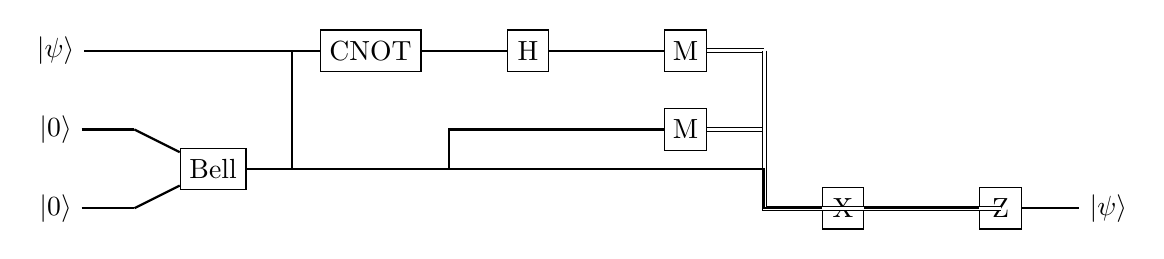
\begin{tikzpicture}
    % Styles
    \tikzset{
        gate/.style={draw, fill=white, minimum size=1.5em},
        wire/.style={thick},
        measure/.style={draw, fill=white, minimum size=1.5em, inner sep=0pt},
        classical/.style={double, double distance=1pt}
    }

    % Qubits
    \node at (0,0) (q1) {$\ket{\psi}$};
    \node at (0,-1) (q2) {$\ket{0}$};
    \node at (0,-2) (q3) {$\ket{0}$};

    % Wires
    \draw[wire] (q1) -- ++(1,0) coordinate (q1end);
    \draw[wire] (q2) -- ++(1,0) coordinate (q2end);
    \draw[wire] (q3) -- ++(1,0) coordinate (q3end);

    % Gates
    \node[gate] at (2,-1.5) (bell) {Bell};
    \draw[wire] (q2end) -- (bell);
    \draw[wire] (q3end) -- (bell);

    \node[gate] at (4,0) (cx1) {CNOT};
    \draw[wire] (q1end) -- (cx1);
    \draw[wire] (bell) -- ++(1,0) |- (cx1);

    \node[gate] at (6,0) (h) {H};
    \draw[wire] (cx1) -- (h);

    \node[measure] at (8,0) (m1) {M};
    \node[measure] at (8,-1) (m2) {M};
    \draw[wire] (h) -- (m1);
    \draw[wire] (bell) -- ++(3,0) |- (m2);

    % Classical wires
    \draw[classical] (m1) -- ++(1,0) coordinate (c1);
    \draw[classical] (m2) -- ++(1,0) coordinate (c2);

    % Correction gates
    \node[gate] at (10,-2) (x) {X};
    \node[gate] at (12,-2) (z) {Z};
    \draw[classical] (c1) -- ++(0,-2) -| (x);
    \draw[classical] (c2) -- ++(0,-1) -| (z);

    % Final state
    \draw[wire] (bell) -- ++(7,0) |- (x);
    \draw[wire] (x) -- (z);
    \draw[wire] (z) -- ++(1,0) node[right] {$\ket{\psi}$};
\end{tikzpicture}

  \subsection{An almost $\QNCon{} = \text{ noisy-}\QNCon{} $.}
  We provide beneath without a formal proof a fault construction that gives an almost \CDO. 
  \begin{enumerate}
    \item We start by initializing many encoded magic states and encoded zeros via the state preparation scheme. Since the block is of length $\log^{\alpha}(n)$, the depth required for that stage is $\log\log(n)$.
    \item In each even step, we apply $\DD$ to keep the error rate low. It fails with probability at most $\Theta\left(\frac{1}{n^k}\right)$, so by the union bound the probability that $\DD$ had at least a single failure is bounded by $\Theta(\frac{1}{n^{k^{\prime}}})$.
    \item We compute the gates over the odd iterations. Each gate is replaced by two applications of gate teleportation, exploiting the magic states. Each application of Clifford, in the second and the first level of the Clifford hierarchy, is followed by $\log(\log (n))$ depth computation for deciding which operation should be applied next.
  \end{enumerate}
  So in overall the depth overhead we get is $\log \log n$, when the battle neack is the time required to decide on the correction \ctt{change term} given the measurement results of the gate teleportation gadget. That raise the question whether there exists Memory codes for which one can perform the correction searching in $O(1)$ depth. 

  \section{ Cues against \CDO.  }\label{sec:passi}

  \section {Applications.} \label{sec:app}

%
%
  %\subsection{Classical and Quantum Circuits.} 
  %\begin{definition}
    %location $(i,j)$ of $C$. \ctt{Add here a figure of classical circuit, that demonstrates locations.}
  %\end{definition}
%
%
  %\subsection{Circuit Classes.}
 %$\QACze$ is the class of decision problems solvable by a family of constant-depth, polynomial-size quantum circuits. Here each layer of the circuit is a tensor product of one-qubit gates and Toffoli gates, or is a tensor product of controlled-NOT gates. 
 %$\QNCze$ Constant-depth quantum circuits without fanout gates.
 %$\QNCon$ Same as QNC, but logarithmic depth instead of polylogarithmic depth.
%
%
%
%
%\subsection{Quantum Codes.} \label{sec:quantum} A quantum code over $n$ qubits is an embedding of $\mathcal{H}_{2}^{\otimes k}$ as a subspace of $\mathcal{H}_{2}^{\otimes n}$. Similar to classical codes, we will call $n$ and $k$ the physical and logical qubits. The embeddings of states in $\mathcal{H}_{2}^{\otimes k}$ are called codewords or encoded states. In addition, we will use the term "logical operator" (i.e. logical $X_{i}$) to describe an operator that acts on the code space exactly as it would act on the logical space $\mathcal{H}_{2}^{\otimes k}$ (in our example, turning on and off the encoded state corresponds to the $i$th qubit exactly as $X_{i}$ acts as Pauli $X$ on the $i$th qubit in $\mathcal{H}_{2}^{\otimes k}$). 
%
%We will denote by $X$ and $Z$ the single $X$ and $Z$ Pauli operators, by $X_{i}$ the application of $X$ on the $i$th qubit and nothing else (identity) on the rest of the qubits. By $X^{(v)}$ for some $v \in \mathbb{F}_{2}^{n}$, we mean the operator composed by applying $X$ on each of the qubits whose index is a non-trivial coordinate of $v$ and identity elsewhere. In a similar fashion, we define $Z^{(v)}$. When the context is clear, we will allow ourselves to omit the brackets, i.e. $Z^{v}$. The weight of a Pauli operator is the number of coordinates on which the operator acts non-trivially. Recall that the set of Pauli $+ I$ spans all the Hermitian matrices. We say that the Pauli weight of an operator is the maximal weight of a Pauli in its Pauli decomposition. For example, consider the operator $A = IXX + ZII$, the weight of $A$ is $2$.
%
%The distance of a quantum code is the minimal weight of an operator that takes one codeword to another. We use the standard bracket notation to describe quantum states and in addition, we define for a vector space $A \subset \mathbb{F}_{2}^{n}$ the notation $\ket{A}$ to represent the uniform superposition of all the vectors belonging to that space, namely: \begin{equation*}
  %\begin{split}
%\ket{A} = \frac{1}{\sqrt{|A|}}\sum_{x \in A}{\ket{x}}
  %\end{split}
%\end{equation*}
%We define in the same way the notation to hold for affine spaces, $\ket{x +A}$. We will use $\propto$ to denote a quantum states up to normalization factor, for example $\ket{\psi} \propto \ket{0} + \ket{1}$ means that $\ket{\psi} = \frac{1}{\sqrt{2}}(\ket{0} + \ket{1})$.
%A CSS code is a quantum code defined by a pair of classical codes $C_{X}$ and $C_{Z}$, satisfying $C_{Z}^{\perp} \subset C_{X}$, such that any codeword of it has the form $\ket{x + C_{Z}^\perp}$, where $x \in C_{X}$. We will use $Q$ to refer to a CSS code in general and use $\QQ$ to refer to the vectors associated with the $X$-generators or the encoded states in the computational basis. In the same way, $C_{Z}/C_{X}^{\perp}$ refers to the $Q$ in the phase basis. We will say that a CSS code $Q$ is a LDPC if $C_{X}$ and $C_{Z}$ are both LDPC codes. Our construction uses the classical Tanner code \cite{Tanner}, the expander codes \cite{ExpanderCodes}, and \Hyp  code (quantum expanders) \cite{Leverrier_2015}, \cite{Tillich_2014}, \cite{overheadofquantumerrorcorrection}. We will not describe these constructions and refer the reader to those papers for further information.
%
%\subsection{Decoders.} \label{sec:decoders} We denote by $C_{g}$ the good qLDPC code \cite{Dinur} \cite{Pavel} \cite{leverrier2022quantum}, and by $C_{ft}$ the concatenation code presented at \cite{aharonov1999faulttolerant} ($ft$ stands for fault tolerance). For a code $C_{y}$, we use $\Phi_{y}, E_{y}, D_{y}$ to denote the channel maps circuits into the their matched circuits compute in the code space, the encoder, and the decoder, respectively. We use $\Phi_{U}$ to denote the 'Bell'-state storing the gate $U$. We say that a state $\ket{\psi}$ is at a distance $d$ from a quantum code $C$ if there exists an operator $U$ that sends $\ket{\psi}$ into $C$ such that $U$ is spanned on Paulis with a degree of at most $d$. Sometimes, when the code being used is clear from the context, we will say that a block $B$ of qubits has absorbed at most $d$ noise if the state encoded on $B$ is at a distance of at most $d$ from that code.
%
%\subsection{Complexity Classes.}
%
%
%
%%(Named in honor of Nick Pippenger.)
%\begin{definition}[$\NC$ - Nick's Class]
%$\NC_i$ is the class of decision problems solvable by a uniform family of Boolean circuits, with polynomial size, depth $O(\log^i(n))$, and fan-in $2$. 
%\end{definition}
%
%\begin{definition}[$\QNC$]
  %The class of decision problems solvable by polylogarithmic-depth, and finate fan out/in quantum circuits with bounded probability of error. Similarly to $\NC_i$, $\QNC_i$ is the class where the decisdes the circuits have $\log^i (n)$ depth.  
%\end{definition}
%
%\begin{definition}[$\QNCG$]
  %For a fixing finate fan in/out gateset $G$, the class with deciding circuits composed only for gates in $G$ and at depath at most polylogaritmic. And in similar to $\QNC_{i}$, $\QNCiG$ is the restirction to circuits with depath at most $\log^{i}(n)$.  
%\end{definition}
%
%\begin{openproblem}
%Consider a fault tolerance scheme $\tilde{C}$ for a logical circuit $C$ which uses the logical gateset $V_{1}, V_{2}, .. V_{t}$. Given a set of fault tolerance logical gates $U_{1}, U_{2}, .. U_{t}$, how would the fault tolerance version of $C$ look when using $U_{1}, U_{2}, .. U_{t}$? Specifically, is rewriting the Solovay-Kitaev again might give a lower depth ciruit?
%\end{openproblem}
%
%\begin{openproblem}
%Given a code with non-trivial distance, what is the complexity of performing gate teleportation, specifically computing the $T$ gate? Or computing a gate which is at the $j$-level of the Clifford hierarchy? What is the classical computation time needed to perform the correction? (Find the right Clifford gate for fixing the computation).
%\end{openproblem}
%
%\begin{openproblem}
  %Is it possible to compute fault tolerance without paying a significant overhead at the depth of the circuits? In particular, Is it $\QNCon \subset \text{noisy}-\QNCon$.
%\end{openproblem}
%
%
%\section{Todo:}
%\begin{enumerate}
  %\item Move to encoding each qubit by logarithmic width (instead of chanks) the reason is that the gate teleportation becomes complicated when it applied over higher dimension. 
  %\item Then showing for 2-qubit gates set that is indeed works.
  %\item Treating separately to noise observed in two qubits gates. 
%\end{enumerate}
%
%
%\section{ The Noise Model } 
%Informally classical noisy circuits describe the running computation of circuits when the bits have probabilities to flip. As exactly to the classical case, in noisy quantum circuits qubits have probabilities to fault. We formalise the noise model by defining a channel $\mathcal{N} : \mathcal{C} \rightarrow \mathcal{D}\left(\mathcal{C}\right)$ that given an ideal circuit induce distribution over circuits. For example, one can consider a Pauli channel, which  after each gate of the original circuit, either do nothing with probability $1-p$ or, with probability $1-p$ impose uniformly one of the Pauli operators $X,Z,Y$. Formally:  
%\begin{definition}
  %Pauli channel $\mathcal{N}: \mathcal{C}\rightarrow \mathcal{D} \left( \mathcal{C} \right)$ defined to give on input $C \in \mathcal{C}$ the distribution over circuits $\tilde{C}$ where any even location of $(i, 2j)$ of $\tilde{C}$ equals to the $(i,j)$ location of $C$, and any odd location $(i,2j+1)$ of $\tilde{C}$ is the density operator $(1-p) I + \frac{p}{3} \left(X + Y + Z  \right)$. 
%\end{definition}
%
%The Pauli channel is charactered by exhibits an independent noise on the qubits, Yet for most of the fault tolerance construction a much more weaker property is required to be assumed. We say that a channel is a local stochastic noise channel if the probability to error to be occur is exponentially decays at the number of qubits the error supports.  
 %
%\begin{definition}
  %An error channel $\mathcal{N}: \mathcal{C}\rightarrow \mathcal{D} \left( \mathcal{C} \right)$ will be said to be a local stochastic noise channel if there exists a constant $c$ such the probability to a fault to be applied on locations $(I ,j)$, where $I$ is a subset of qubits, is less than $c^{-n}$.
%\end{definition}
%
%Another important property of a noise model which we consider in this work is the accessibility to fresh qubits, also known as resets gate. When having an access to fresh qubits one can assume that in any time in the computation there are qubits at the $\ket{0}$ states. Usually those qubits are used to measured the syndrome relative to an error correction code. It was proven that without an access to fresh qubits quantum circuits cannot last than logarithmic depth without mixing into a fully mixed state, meaning to be turned into complete garbage \cite{aharonov1996limitationsnoisyreversiblecomputation}. That result also holds for a classical noisy computation. 
%
%\begin{definition}
  %An error channel $\mathcal{N}: \mathcal{C}\rightarrow \mathcal{D} \left( \mathcal{C} \right)$ will be said to has a fresh qubits access if location $(i,j)$ in an output gate $\tilde{C}$ has a non zero probability to exhibits a fault if there is a $j^{\prime} < j$ such a location $(i, j^{\prime})$ such that on the input circuit $C$, at location $(i,j^{\prime})$ a non identity gate is posed.     
%\end{definition}
%
%We close this section by formalize the \noiseQNCon class. 
%\begin{definition}
  %We denote by \noiseQNCon the class of decision problems solvable by logarithmic-depth quantum circuits, subjected to a local stochastic noise,  with bounded probability of error. 
%\end{definition}
%We mention that in \cite{aharonov1996limitationsnoisyreversiblecomputation}, it was proved how a fault tolerance circuit with an access to fresh qubits, at logarithmic depth, can be converted to a log depth circuits without a fresh qubits access at the cost which is at most polynomial in wide. Meaning that Proving that $ \QNCon \subset $ \noiseQNCon implies also that $ \QNCon $ can be computed, in the presence of noise without an access to fresh qubits. 
%
%
%\section{ Fault Tolerance (With Resets gates) at Linear Depth. } 
%
%\begin{claim}
%There exists a value $p_{th} \in (0,1)$ such that if $p < p_{th}$, then any quantum circuit $C$ with a depth of $D$ and a width of $W$ can be computed by a $p$-noisy circuit $C^{\prime}$, which allows for resets. The depth of $C^{\prime}$ is at most $\max{ \{O(D), O(\log(WD)) \} }$.
%\end{claim}
%
%
%\subsection{Initializing Magic for Teleportation gates and encodes ancillaries.}
%The Protocol: \begin{enumerate}
  %\item Initialization of zeros: The qubits are divided into blocks of size $|B|$. Each block is encoded in $C_{g}$ using $D_{ft} \Phi_{ft}[E_{g}] \ket{0^{|B|}}$.
  %\item Initialization of Magic for Teleportation gates: The gates in the original circuit are encoded in $C_{g}$ using $D_{ft} \Phi_{ft}[E_{g}] \ket{\Phi_{U}}$.
  %\item Gate teleportation: Each gate in the original circuit is replaced by a gate teleportation.
  %\item Error reduction: After the initialization step, at each time tick, each block runs a single round of error reduction.
%\end{enumerate}
%
%\begin{claim}[From \cite{leverrier2022decodingquantumtannercodes}]
  %\label{claim:error} 
  %Assuming that an error $|e| \le \gamma n $, i.e $e$ is supported on less than $\gamma n$ bits, then a single correction round reduce $e$ to an error $e^\prime$ such that $|e^{\prime}| < \nu |e|$. 
%\end{claim}
 %%Recall that by definition, $D_{i}E_{i} = I$, or in other words, $D_{i}= E_{i}^{\dagger}$.  
%\begin{claim}
  %\label{claim:noisepa}
  %The gate $ D_{ft} \Phi_{ft}[E_{g}]$ initializes states encoded in $C_{g}$ subject to a $3p$-noise channel.  
%\end{claim}
%\begin{proof}
  %Clearly, with high probability, $\Phi_{ft}[E_{g}]$ successfully encodes into $C_{ft} \circ C_{g}$, let's say with probability $1 - \frac{1}{poly(n)}$. Denote by $E_{i}$ and $D_{i}$ the encoder and decoder at the $i$th level of the concatenation construction. Consider the decoder under $\mathcal{N}$ action: $P_{2}D_{1}P_{2}D_{2},..,P_{i-1}D_{i}P_{i}$, by the fault-tolerance construction, a logical error at the $i$th stage occurs with probability $p^{2^{i}}$. Therefore, by the union bound, the probability that in one of the steps the circuit absorbs an error that is not corrected is less than $p + p^{2} + p^{4} + .. < 2p$. Hence, any decoded qubit absorbs noise with probability less than $2p$.
%
%
  %Thus, overall, we can bound the probability of a single qubit being faulty by:
  %\begin{equation*}
    %\begin{split}
      %\prb{\text{fault} } &=  \prb{\text{fault} |  \Phi_{ft}[E_{g}] }\cdot \prb{\Phi_{ft}[E_{g}]} + \prb{\text{fault} | \overline{\Phi_{ft}[E_{g}]} }\cdot \prb{\overline{\Phi_{ft}[E_{g}]}}\\
      %&\le  \prb{\text{fault} |  \Phi_{ft}[E_{g}] } + \prb{\overline{\Phi_{ft}[E_{g}]}} \le 2p + \frac{1}{poly(n)} \le 3p
    %\end{split}
  %\end{equation*}
%
  %\begin{remark}
%In our construction, we use the concatenation code to encode blocks of length $\log(n)$. Therefore, any $poly(n)$ in the above should be replaced by $\log(n)$. However, this does not affect anything since the inequality does not depend on $n$.
  %\end{remark}
%
%%
%%
%%  \begin{equation*}
%%    \begin{split}
%%      \mathcal{N}(D) &= \left((\mathcal{N}(D))^{\dagger}\right)^{\dagger} =  \left(\sum_{P_{1}, P_{2}, .., P_{i} \in \mathcal{P}}{ \prb{P_{1}, P_{2}, .., P_{i}}  \left(D_{1}P_{2}D_{2},..,P_{i-1}D_{i}P_{i}\right)^{\dagger}} \right)^{\dagger} \\ 
%%      &= \left( \sum_{P_{1}, P_{2}, .., P_{i} \in \mathcal{P}}{ \prb{P_{1}, P_{2}, .., P_{i}}  P_{i}E_{i}P_{i-1}E_{i-1},..,P_{1}E_{1} } \right)^{\dagger}\\
%%      &= \left( \left( 1 -\frac{1}{poly(n)} \right)\sum_{P_{i} \in \mathcal{P}}\prb{P_{i}}P_{i}E + \frac{1}{poly(n)} A  \right)^{\dagger} \\ 
%%      &= \left( 1 -\frac{1}{poly(n)} \right)\sum_{P_{i} \in \mathcal{P}}\prb{P_{i}}DP_{i} + \frac{1}{poly(n)} A 
%%\end{split}
%%  \end{equation*}
%%
%%  %Since $D$ is semi-transversal gate, it preserves the 
%%
%%
%%  And notice that $\star$ is with probability $1 - \frac{1}{poly(n)}$ equals to $E_{i}E_{i-1}..,E_{1}=E$. Hence $\mathcal{N}(D)$ equals to $\left( P E \right)^{\dagger} = PD$.
%%
%%  \begin{equation*}
%%    \begin{split}
%%      \braket{ \psi^{\prime} | P_{i}E_{i}P_{i-1}E_{i-1},..,P_{1}E_{1} \psi } = \braket{ \psi^{\prime} P_{i}D_{i}P_{i-1}D_{i-1},..,P_{1}D_{1} | \psi }
%%    \end{split}
%%  \end{equation*}
%%  Thus for any pauli-channel $\mathcal{N} : L(H) \rightarrow L(H)$, and $\psi^{\prime}$ which is a codeword we get: 
%%  \begin{equation*}
%%    \begin{split}
%%      \braket{ \psi^{\prime} \mathcal{N}(D) | \psi } &=  \sum_{P_{1}, P_{2}, .., P_{i} \in \mathcal{P}}{ \prb{P_{1}, P_{2}, .., P_{i}}  \braket{ \psi^{\prime} P_{i}D_{i}P_{i-1}D_{i-1},..,P_{1}D_{1} | \psi }} \\
%%      &=  \sum_{P_{1}, P_{2}, .., P_{i} \in \mathcal{P}^{\star}}{  \prb{P_{1}, P_{2}, .., P_{i}}\braket{ \psi^{\prime} | P_{i}E_{i}P_{i-1}E_{i-1},..,P_{1}E_{1} \psi }} \pm O(  \frac{1}{poly(n)})\\
%%      &=  \sum_{P_{1}, P_{2}, .., P_{i} \in \mathcal{P}^{\star}}{  \prb{P_{1}, P_{2}, .., P_{i}}\braket{ \psi^{\prime} | P_{i} E \psi }} \pm O(  \frac{1}{poly(n)})\\
%%      &\le  \sum_{ P_{i} \in \mathcal{P}}{  \prb{ P_{i}}\braket{ \psi^{\prime} | P_{i} E \psi }} \pm O(  \frac{1}{poly(n)}) \\
%%      &\le  \sum_{ P_{i} \in \mathcal{P}^{\le d}}{  \prb{ P_{i}}\braket{ \psi^{\prime} | P_{i} E \psi }} \pm O (e^{-d \cdot n} ) \pm O(  \frac{1}{poly(n)}) \\
%%      & \le   \sum_{ P_{i} \in \mathcal{P}/\mathcal{P}^{\star}}{  \prb{ P_{j} \in B_{d}\left( P_{i} \right)}\braket{ \psi^{\prime} | P_{i} E \psi }}  \pm O (e^{-d \cdot n} ) \pm O(  \frac{1}{poly(n)}) 
%%    \end{split}
%%  \end{equation*}
%%  Using the fact that the concatenation code is monotonic (\Cref{def:mono}) we get that the probability to have physical fault $P_{j}$.   
%%%\end{widetext}
%\end{proof}
%
%\begin{claim}
  %\label{claim:prob}
  %With a probability $ 1 - \frac{WD}{|B|} \cdot D 2e^{-2|B|(\beta - p)} $, the total amount of noise absorbed in a block at any given time $t$, is less than $\gamma n$. 
%\end{claim}
%\begin{proof}
%Consider the $i$th block, denoted by $B_{i}$. By applying Hoeffding's inequality, we have that the probability that more than $\beta |B|$ qubits are flipped at time $t$ is less than $2e^{-2|B|(\beta - p)}$. By using the union bound over all blocks at all time locations, we can conclude that with probability $1 - \frac{WD}{|B|} \cdot D 2e^{-2|B|(\beta - p)}$, the noise absorbed in a block is less than $|\beta|B$ for the entire computation.
%
%Let $X_{t}$ denote the support size of the error over $B_{i}$ at time $t$. Using \Cref{claim:error}, we can bound the total amount of error absorbed by a block until time $t$ as follows:
%\begin{equation*}
%\begin{split}
%X_{t} \le \nu \cdot (X_{t-1} + \beta |B| ) \le \nu(\gamma+\beta) |B| \le \gamma |B|
%\end{split}
%\end{equation*}
%\end{proof}
%
%
%\begin{claim}
  %The total depth of the circuit is $O ( D  ) + O ( \log^{c} |B| )$. 
%\end{claim}
%\begin{proof}
  %The gate for encoding $|B|$-length blocks in $C_{g}$ is a Clifford gate and can therefore be computed in $O(\log|B|)$ depth. The encoding of the magic/bell states is done by first computing them in the logical space (un-encoded qubits) and then encode them using the encoder. Hence, the fault-tolerant version of both initializing ancillaries and magic states/bell states costs $O( (\log |B|) \cdot \log^{c}( |B| \log |B| ) )$ \footnote{The width of the original circuit is $|B|^{2}$ so the number of locations is $ |B|^{2} \cdot \log |B|$} depth \cite{aharonov1999faulttolerant}. Backing into $C_{g}$ from $C_{ft}$ by decoding the concatenation code takes exactly as long as the encoding, namely $O( (\log |B|) \cdot \log^{c}( |B| \log |B| ) )$.
%
  %Then, using the bell measurements, any of the logical gates takes $O(1)$ depth. Since we only perform a single round of error correction, the remaining computation until the last decoding stage takes at most constant time of the original depth. Finally, we pay $O(\log |B|)$ for complete decoding. Summing all, we get: 
  %\begin{equation*}
    %\begin{split}
     %&  O ( \log |B|\cdot  \log^{c}( |B| \log |B| ) )  + O ( D  ) + O ( \log |B| ) \\ 
     %= & O ( D  ) + O ( \log^{c} |B| )
    %\end{split}
  %\end{equation*}
%\end{proof}
%
%Assuming that $W$ is polynomial in $D$, taking the block length to be $|B| = \log((W \cdot D)^c)$, as shown in \Cref{claim:prob}, results in a linear fault tolerance construction with a success probability of $1 - \frac{1}{\log^{c_2}(W \cdot D)}$. This means that the fault tolerance version of circuits in $\textbf{QNC}_1$ has a logarithmic depth. Additionally, using the construction in \cite{aharonov1996limitationsnoisyreversiblecomputation} produces a polynomial fault tolerance circuit in the reversible gates setting. \ctt{ We missed the fact that it requires non trivial classical computation to compute what gate should be applied after the gate teleportation (i.e $UPU^{\dagger}$ )}.
%
%
%
%
%\section{ $\QACze \subset $\noiseQNCon }
%For completing this one has to show that one can compute the parity with a fixed gates set. Here is what we need: 
%\begin{enumerate}
  %\item having the logical states $\ket{0} + e^{i\frac{|x|}{2^{j}}}\ket{1}$
  %\item Note that gate $\ket{0} + e^{i\frac{1}{2^{j}}}\ket{1}$ is in the $j$th level of the Clifford. Yet after getting the Pauli one has to compute what gate should be applied. And when considering logical space it's not a constant operation, yet it could computed in the logical space, so what we need is just to look, so for a $m$-length code, $\log m$. Or maybe can we do better?   
  %\item if the diminution of the code is constant?  
    %\begin{equation*}
      %\begin{split}
	%& \ket{C_{Z}^{\perp}, C_{Z}^{\perp}} + \ket{C_{Z}^{\perp} + 1_{L}, C_{Z}^{\perp} + 1_{L}} \\ 
	%\rightarrow  \alpha  & \ket{C_{Z}^{\perp}} \left( \ket{C_{Z}^{\perp}, C_{Z}^{\perp}} + \ket{C_{Z}^{\perp} + 1_{L}, C_{Z}^{\perp} + 1_{L}} \right) \\
	%+   \beta & \ket{ C_{Z}^{\perp} + 1_{L}}\left( \ket{C_{Z}^{\perp}+1_{L}, C_{Z}^{\perp}} + \ket{C_{Z}^{\perp}, C_{Z}^{\perp} + 1_{L}} \right)
      %\end{split}
    %\end{equation*}
%\end{enumerate}
%
%
%\section{ Does $\NCon \subset $\noiseQNCon ?}
%
%
%\section{ Does Factoring $\subset$ \noiseQNCon ?}
%
%\begin{equation*}
  %\begin{split}
    %D(n) &= \Theta(\log n ) + D(\sqrt{n})\\
    %\Rightarrow D(n) & = \Theta( \log n ) 
  %\end{split}
%\end{equation*}
%
%
%
%
\printbibliography
\end{document}


